\documentclass[parskip=half,DIV=12,bookmarkpackage=false]{scrartcl}

\title{Lab assignment 1}
\subtitle{ATM S 544}
\author{Dominik Stiller}
\date{\today}

\usepackage[english]{babel}
\usepackage[utf8]{inputenc}
\usepackage{siunitx,amsmath,physics}
\usepackage{caption,subcaption,graphicx,csquotes,xcolor}
\usepackage{booktabs}
\usepackage{placeins}
\usepackage[
	backend=biber,
	bibwarn=true,
	bibencoding=utf8,
	sortlocale=en_US,
	url=false,
	style=apa,
	isbn=false
]{biblatex}

\definecolor{uw-purple}{RGB}{51, 0, 111}

\usepackage{hyperref}
\hypersetup{
	% hidelinks,
	colorlinks=true,
	linkcolor=black,
	citecolor=black,
	urlcolor=uw-purple
}

\usepackage{doi}
\usepackage{nomencl}
\makenomenclature
\usepackage[noabbrev,capitalise]{cleveref}
\usepackage[acronym,nonumberlist,nopostdot,nogroupskip]{glossaries}
\usepackage[
	outputdir=build,
]{minted}
\setminted{
	linenos,
	tabsize=4,
	fontsize=\small,
}
\newmintinline{python}{}

\usepackage{lmodern}
\usepackage[T1]{fontenc}
\usepackage{inconsolata}
\usepackage{tikz}

\newcommand{\result}[1]{\colorbox{uw-purple}{\textcolor{white}{#1}}}

\setlength{\nomlabelwidth}{1.5cm}
\setlength{\nomitemsep}{-\parsep}
\newcommand{\nomunit}[1]{%
\renewcommand{\nomentryend}{\hspace*{\fill}\si{#1}}}

\sisetup{per-mode=symbol}
\AtBeginDocument{\RenewCommandCopy\qty\SI}

\DeclareGraphicsRule{.ai}{pdf}{.ai}{}

\addbibresource{bibliography.bib}



\begin{document}

\maketitle

\vfill

\section{Analysis of ensemble differences}

The initial conditions of the two ensemble members have a Z500 geopotential RMS difference of 0.05003. This is to be expected since it is the noise amplitude we set to induce ensemble spread. For finer grids, the value would approach exactly 0.05 by the law of large numbers.

\begin{figure}[h]
    \centering
    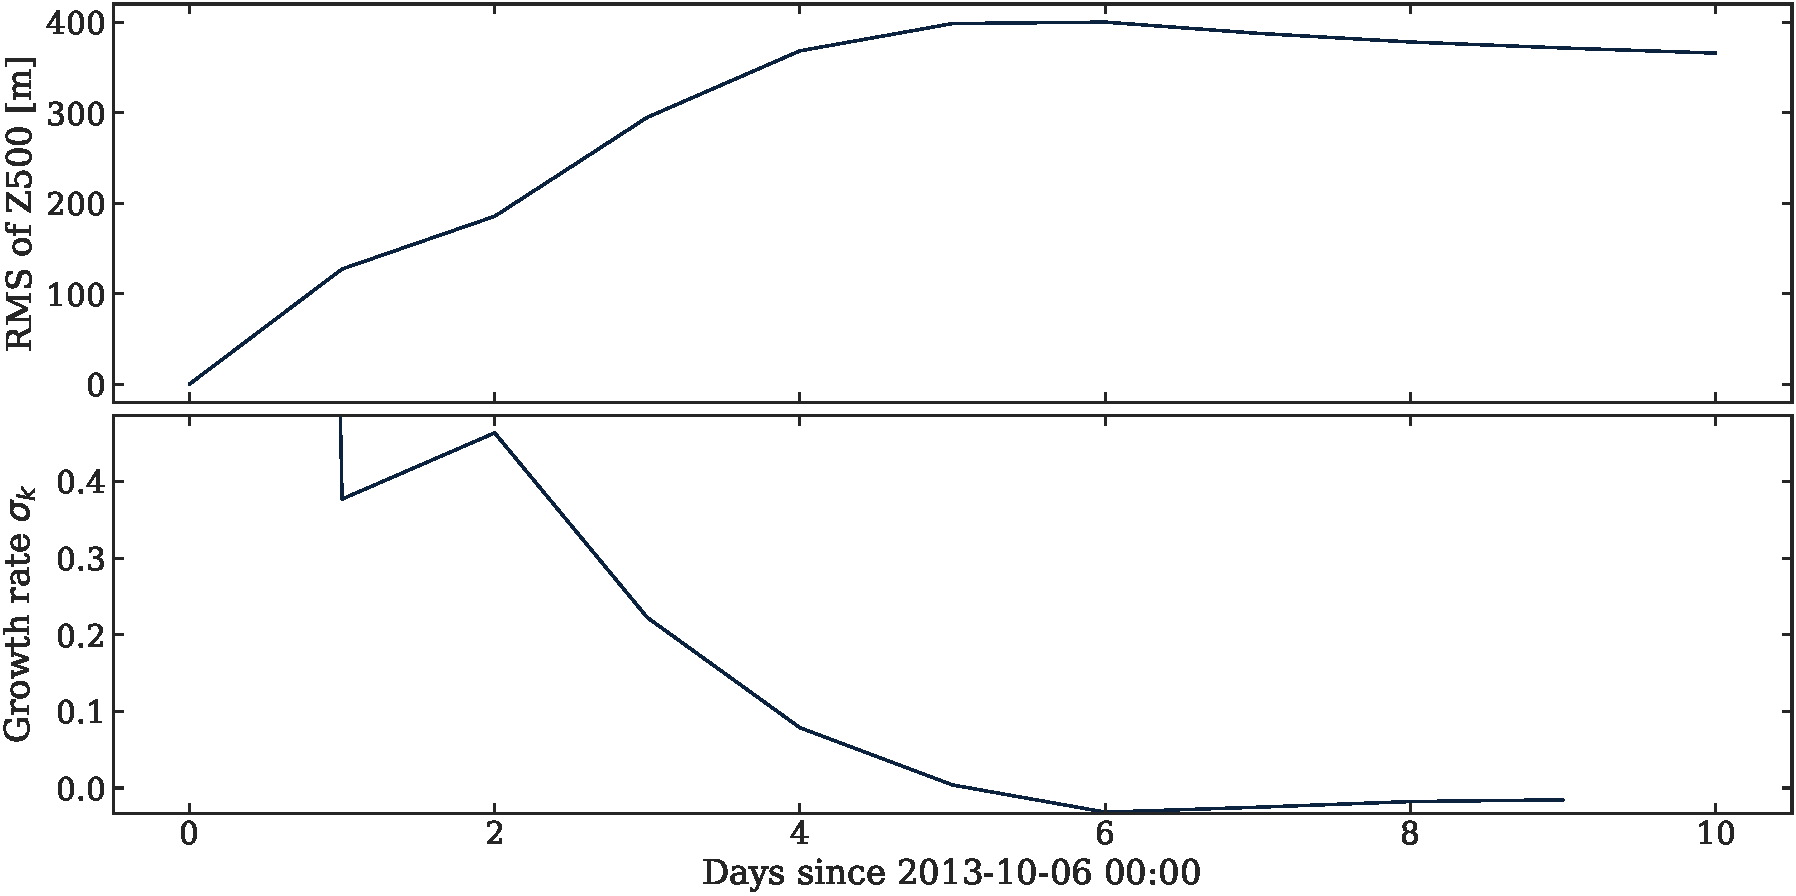
\includegraphics[width=\textwidth]{figures/factor1.pdf}
    \caption{Difference between ensemble Z500 height for baseline noise.}
    \label{fig:fac-1}
\end{figure}

\cref{fig:fac-1} shows the geopotential \emph{height} RMS difference and daily growth rate for a noise amplitude of 0.05. The two members diverge for the first four to five days, then settle around an RMS difference of \qty{360}{m} with $|\sigma_k| \approx \num{e-2}$. During the divergence period, small-scale differences propagate and lead to large-scale differences. Once the members settle on a large-scale structure, they do not diverge further on the timescale of ten days \emph{in a mean sense}. While the RMS decreases slightly for longer lead times, further experiments would be necessary to see if the trend continues beyond ten days.


\newpage
\begin{figure}[h]
    \centering
    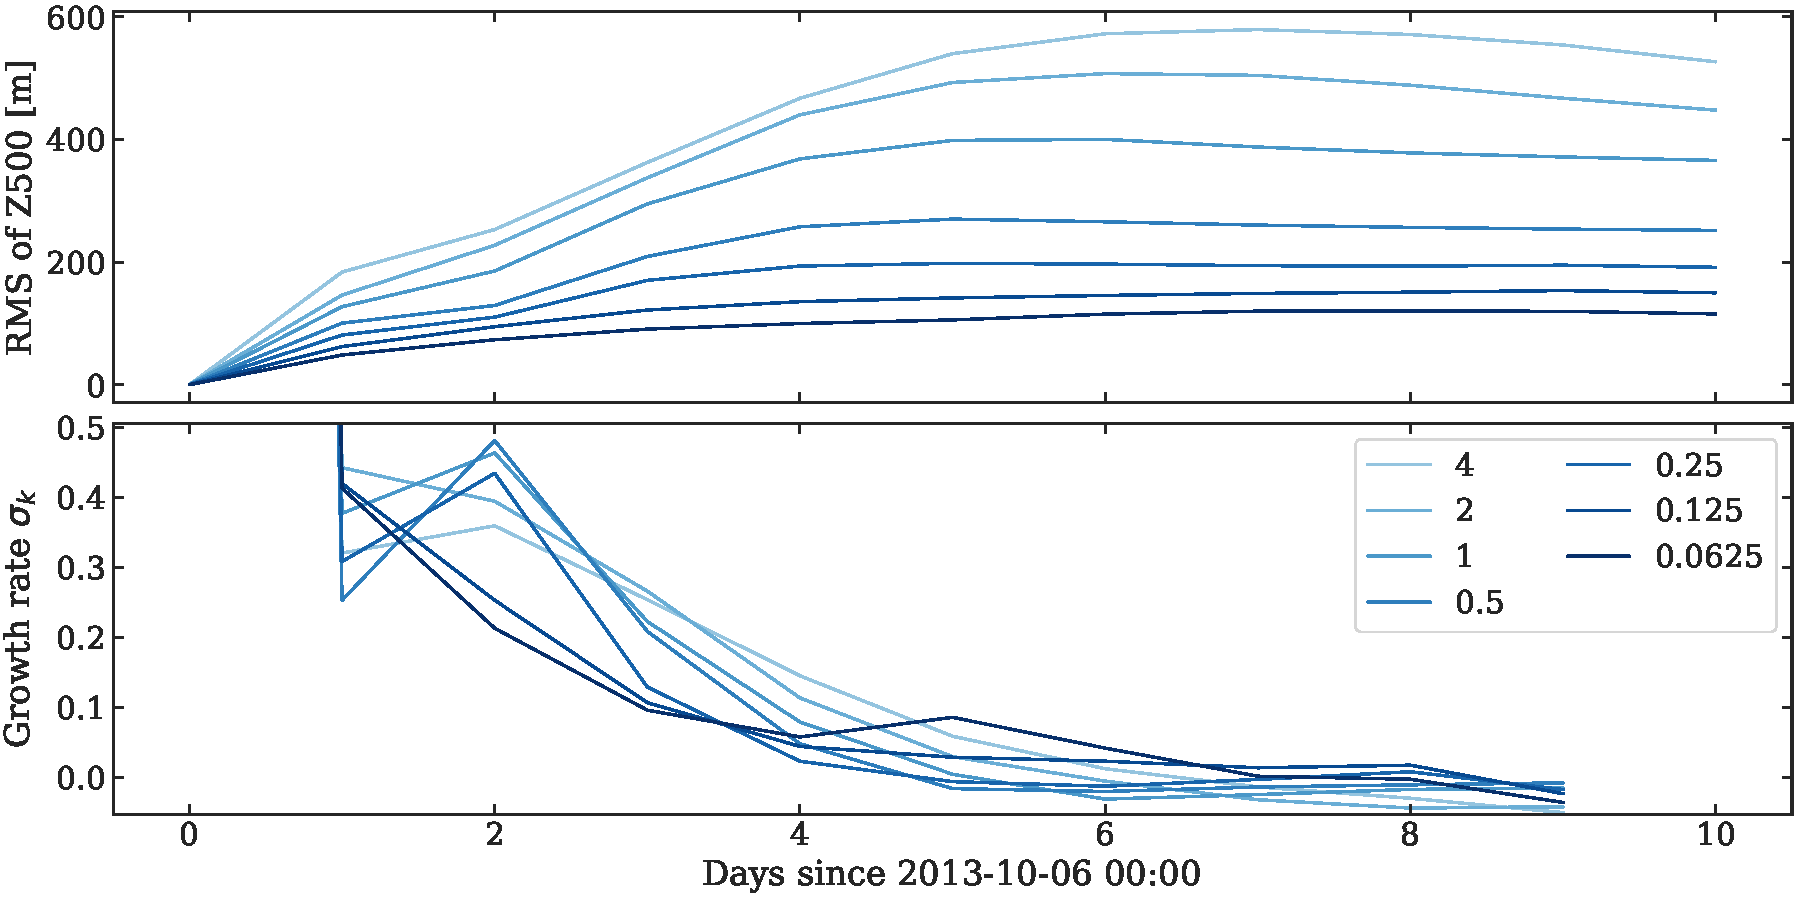
\includegraphics[width=\textwidth]{figures/all_factors.pdf}
    \caption{Difference between ensemble Z500 height for different noise levels.}
    \label{fig:fac-all}
\end{figure}

\cref{fig:fac-all} shows the same metrics but the noise amplitude of 0.05 is scaled by factors between 1/16 and 4. Larger perturbation amplitudes lead to greater divergence between the ensemble members, although not proportional to the scaling factor. Alse, the initial growth rate is slightly smaller for higher noise amplitudes, but they seem to approach the same limit of $|\sigma_k|$. That larger perturbations lead to more initial divergence can be shown, for example, from the Taylor series expansion about the unperturbed initial condition. Therefore, the noise amplitude is instrumental for controlling ensemble spread and matching it to true atmospheric uncertainty.



\end{document}
